\usepackage{xcolor}
\usepackage{afterpage}
\usepackage{pifont,mdframed}
\usepackage[bottom]{footmisc}


\createsection{\Grader}{Grader di prova}

\renewcommand{\inputfile}{\texttt{stdin}}
\renewcommand{\outputfile}{\texttt{stdout}}
\makeatletter
\renewcommand{\this@inputfilename}{\texttt{stdin}}
\renewcommand{\this@outputfilename}{\texttt{stdout}}
\makeatother

% % % % % % % % % % % % % % % % % % % % % % % % % % % % % % % % % % % % % % % % % % %
% % % % % % % % % % % % % % % % % % % % % % % % % % % % % % % % % % % % % % % % % % %

Cecilia è l'ambientalista delle OII, sempre attenta al rispetto dell'ambiente e
alla raccolta differenziata. Naturalmente, a casa Cecilia possiede un orto: una
lunga striscia di terra rettilinea in cui sono piantati $N$ semi. Ogni seme è
stato piantato ad una certa distanza dall'inizio $X_i$ e ad una certa profondità
$P_i$. Tutti i valori sono espressi in millimetri: i semi però, per motivi
logistici sono sempre piantati in posizioni multiple di $1$cm (i valori di $X_i$
e $P_i$ sono quindi garantiti essere multipli di $10$).

Per bagnare i suoi semi, Cecilia installerà degli irrigatori lungo la superficie
del campo. Questi spruzzeranno acqua che, grazie alla permeabilità del terreno,
raggiungerà la terra in profondità. Quando un irrigatore verrà acceso, l'acqua
spruzzata si espanderà sulla superficie con una velocità di $1$ millimetro al
secondo verso destra e verso sinistra. I punti così bagnati, a loro volta, si
espanderanno verso il basso alla stessa velocità. Questo andrà a formare un'area
bagnata triangolare:%
%
\begin{figure}[H]
  \centering
  \includegraphics[width=.78\linewidth]{asy_orticoltura/fig0.pdf}
  \caption{Due irrigatori in posizioni $38$mm e $70$mm, accesi per $26$s e $20$s rispettivamente.}
\end{figure}

Per esempio, in Figura 1 i due semi più a destra sono bagnati, mentre il seme di sinistra non lo è. Notare che gli irrigatori non si influenzano a vicenda.
Più precisamente, indicando con $(X_{seme}, P_{seme})$ le coordinate di un seme,
con $X_{irrigatore}$ la posizione di un irrigatore e con $T_{irrigatore}$ il suo
tempo di accensione, avremo che il seme è bagnato quando:

$$|X_{seme}-X_{irrigatore}| + P_{seme} \le T_{irrigatore}$$

Ogni irrigatore comporta per Cecilia un costo fisso di $C$ centesimi di euro per
l'acquisto ed un costo variabile di $1$ centesimo per ogni secondo di utilizzo.
Gli irrigatori possono essere temporizzati in modo da essere accesi per tempi
variabili, ma sempre multipli di $1$ secondo. Devono inoltre essere posizionati
a distanze multiple di $1$mm.

Aiuta Cecilia ad acquistare, posizionare e temporizzare gli irrigatori in modo
da minimizzare il costo totale dell'impianto, riuscendo a bagnare tutti i semi!

% % % % % % % % % % % % % % % % % % % % % % % % % % % % % % % % % % % % % % % % % % %
% % % % % % % % % % % % % % % % % % % % % % % % % % % % % % % % % % % % % % % % % % %


\Implementation

Dovrai sottoporre un unico file, con estensione \texttt{.c} o \texttt{.cpp}.

\begin{warning}
Tra gli allegati a questo task troverai un template \texttt{orticoltura.c} o
\texttt{orticoltura.cpp} con un esempio di implementazione.
\end{warning}

Dovrai implementare la seguente funzione:

\begin{center}\begin{tabularx}{\textwidth}{|c|X|}
\hline
C    & \verb|void irriga(int C, int N, int* X, int* P);|\\
C++  & \verb|void irriga(int C, int N, vector<int>& X, vector<int>& P);|\\
\hline
\end{tabularx}\end{center}

\begin{itemize}[nolistsep]
  \item L'intero $C$ è il costo fisso relativo ad un irrigatore.
  \item L'intero $N$ rappresenta il numero di semi nel campo.
  \item L'array \texttt{X}, indicizzato da $0$ a $N-1$, contiene l'elenco delle posizioni dei semi piantati.
  \item L'array \texttt{P}, indicizzato da $0$ a $N-1$, contiene l'elenco delle profondità dei semi piantati.
\end{itemize}

\medskip

Il tuo programma potrà utilizzare le seguenti funzioni, già definite nel grader:

\begin{center}\begin{tabularx}{\textwidth}{|c|X|}
\hline
C/C++  & \verb|void posiziona(int D, int T);|\\
\hline
\end{tabularx}\end{center}

\begin{itemize}[nolistsep]
  \item L'intero $D > 0$ indica la posizione dove verrà installato l'irrigatore.
  \item L'intero $T > 0$ rappresenta il tempo di utilizzo dell'irrigatore.
\end{itemize}

\medskip

\begin{center}\begin{tabularx}{\textwidth}{|c|X|}
\hline
C/C++  & \verb|void budget(int B);|\\
\hline
\end{tabularx}\end{center}

\begin{itemize}[nolistsep]
  \item L'intero $B$ indica il minimo costo di un impianto che bagna tutti i
  semi.
\end{itemize}

\medskip

Il grader chiamerà la funzione \texttt{irriga}. Al suo interno potrai effettuare
chiamate alla funzione \verb|posiziona| per posizionare gli irrigatori e
chiamare la funzione \verb|budget| per restituire il minimo costo dell'impianto.
L'ordine delle chiamate a \verb|posiziona| è irrilevante. In caso di chiamate
multiple alla funzione \verb|budget| verrà considerata solo l'ultima.

% % % % % % % % % % % % % % % % % % % % % % % % % % % % % % % % % % % % % % % % % % %
% % % % % % % % % % % % % % % % % % % % % % % % % % % % % % % % % % % % % % % % % % %

\Grader

Nella directory relativa a questo problema è presente una versione semplificata
del grader usato durante la correzione, che potete usare per testare le vostre
soluzioni in locale. Il grader di esempio legge i dati da \inputfile{}, chiama
le funzioni che dovete implementare e scrive su \outputfile{}, secondo il
seguente formato.

Il file di input è composto da $N+1$ righe, contenenti:
\begin{itemize}[nolistsep,itemsep=2mm]
\item Riga $1$: l'intero $C$, il costo di un irrigatore.
\item Riga $2$: l'intero $N$, il numero di semi.
\item Righe $3\ldots N+2$: i valori \texttt{X[$i$]} e \texttt{P[$i$]} per $i = 0\ldots N-1$.
\end{itemize}

Il file di output è composto da $K+2$ righe, contenenti:
\begin{itemize}[nolistsep,itemsep=2mm]
\item Riga $1$: l'intero $B$, il costo dell'impianto trovato.
\item Riga $2$: l'intero $K$, il numero di irrigatori utilizzati.
\item Righe $3\ldots K+2$: i valori \texttt{D[$j$]} e \texttt{T[$j$]} per $j = 0\ldots K-1$.
\end{itemize}

% % % % % % % % % % % % % % % % % % % % % % % % % % % % % % % % % % % % % % % % % % %
% % % % % % % % % % % % % % % % % % % % % % % % % % % % % % % % % % % % % % % % % % %


\Constraints

\begin{itemize}[nolistsep, itemsep=2mm]
	\item $0 \le C \le 10^9$.
	\item $1 \le N \le 1\,000\,000$.
	\item $10 \le X_i, P_i \le 10^9$ e sono multipli di $10$, per ogni $i=0\ldots N-1$.
	\item Non ci sono mai due semi alla stessa posizione e alla stessa profondità.
\end{itemize}

% % % % % % % % % % % % % % % % % % % % % % % % % % % % % % % % % % % % % % % % % % %
% % % % % % % % % % % % % % % % % % % % % % % % % % % % % % % % % % % % % % % % % % %

\pagebreak

\Scoring

Il tuo programma verrà testato su diversi test case raggruppati in subtask.
Per ogni test case, il punteggio è suddiviso in due parti:

\begin{itemize}[nolistsep,itemsep=2mm]
  \item $60\%$: assegnato se il costo restituito da \verb|budget| è il minimo per cui puoi bagnare tutti i semi;
  \item $40\%$: assegnato se le chiamate a \verb|posiziona| posizionano gli irrigatori in modo ottimo.
\end{itemize}

Il punteggio relativo ad un subtask è pari al punteggio del subtask, moltiplicato per il \textbf{minimo} punteggio ottenuto su un suo test case.

\begin{itemize}[nolistsep,itemsep=2mm]
  \item \textbf{\makebox[2cm][l]{Subtask 1} [\phantom{0}0 punti]}: Casi d'esempio.
  % esponenziale becera
  \item \textbf{\makebox[2cm][l]{Subtask 2} [\phantom{0}5 punti]}: $N \leq 4$, $X_i \leq 100$, $P_i = 10$.
  % dinamica O(N²) senza profondità
  \item \textbf{\makebox[2cm][l]{Subtask 3} [15 punti]}: $N \leq 1000$ e $P_i = 10$.
  % nessun problema di arrotondamento
  \item \textbf{\makebox[2cm][l]{Subtask 4} [20 punti]}: $P_i = 10$.
  % dinamica O(N²)
  \item \textbf{\makebox[2cm][l]{Subtask 5} [20 punti]}: $N \leq 1000$.
  % merge dei triangoli
  \item \textbf{\makebox[2cm][l]{Subtask 6} [20 punti]}: $C = 0$.
  % merge dei triangoli + traslazione / dinamica / greedy sortando per X-P
  \item \textbf{\makebox[2cm][l]{Subtask 7} [20 punti]}: Nessuna limitazione specifica.
\end{itemize}

% % % % % % % % % % % % % % % % % % % % % % % % % % % % % % % % % % % % % % % % % % %
% % % % % % % % % % % % % % % % % % % % % % % % % % % % % % % % % % % % % % % % % % %


\Examples

\begin{example}
\exmpfile{orticoltura.input0.txt}{orticoltura.output0.txt}%
\exmpfile{orticoltura.input1.txt}{orticoltura.output1.txt}%
\end{example}

% % % % % % % % % % % % % % % % % % % % % % % % % % % % % % % % % % % % % % % % % % %
% % % % % % % % % % % % % % % % % % % % % % % % % % % % % % % % % % % % % % % % % % %


\Explanation

Nel \textbf{primo caso di esempio} una soluzione è la seguente: \\[-22pt]
%
\begin{center}
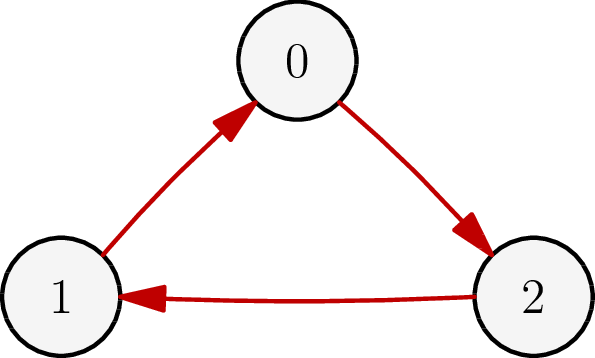
\includegraphics[width=.8\linewidth]{asy_orticoltura/fig1.pdf}
\end{center}

Nel \textbf{secondo caso di esempio} una soluzione è la seguente:
%
\begin{center}
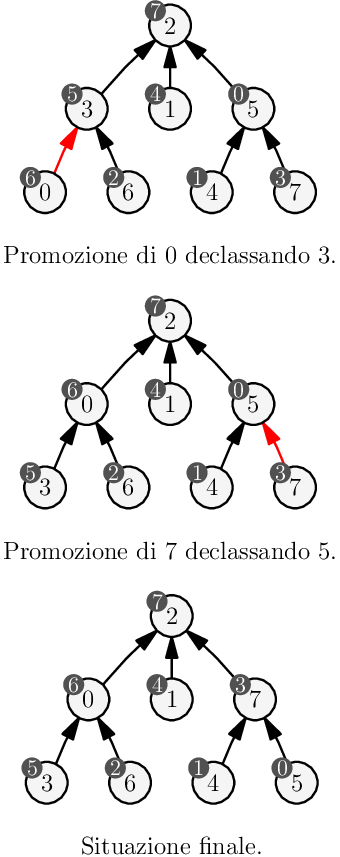
\includegraphics[width=.8\linewidth]{asy_orticoltura/fig2.pdf}
\end{center}
